\documentclass{standalone}
\usepackage{tikz}
\usepackage{graphicx}

\begin{document}\hspace{6cm}
	
	
	
	
	\tikzset{every picture/.style={line width=0.75pt}} %set default line width to 0.75pt        
	
	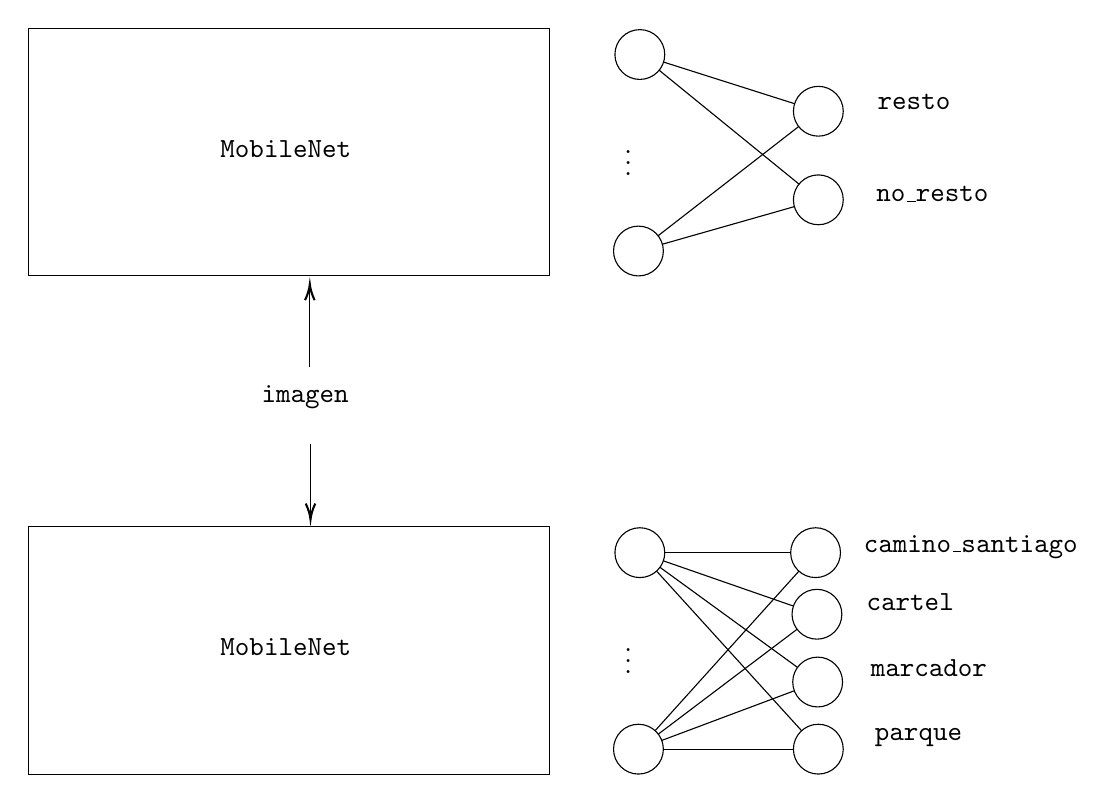
\begin{tikzpicture}[x=0.75pt,y=0.75pt,yscale=-1,xscale=1]
		%uncomment if require: \path (0,458); %set diagram left start at 0, and has height of 458
		
		%Straight Lines [id:da3782540145657389] 
		\draw    (406,97) -- (492,167) ;
		%Shape: Rectangle [id:dp7793126827918091] 
		\draw   (111.33,84.33) -- (362.33,84.33) -- (362.33,203.67) -- (111.33,203.67) -- cycle ;
		%Straight Lines [id:da9688268515745138] 
		\draw    (406,97) -- (492,124.33) ;
		%Straight Lines [id:da4443636790807173] 
		\draw    (405.33,191.67) -- (492,167) ;
		%Straight Lines [id:da6474624574262169] 
		\draw    (492,124.33) -- (405.33,191.67) ;
		%Shape: Circle [id:dp20535554334044726] 
		\draw  [fill={rgb, 255:red, 255; green, 255; blue, 255 }  ,fill opacity=1 ] (480,124.33) .. controls (480,117.71) and (485.37,112.33) .. (492,112.33) .. controls (498.63,112.33) and (504,117.71) .. (504,124.33) .. controls (504,130.96) and (498.63,136.33) .. (492,136.33) .. controls (485.37,136.33) and (480,130.96) .. (480,124.33) -- cycle ;
		%Shape: Circle [id:dp3931688548250376] 
		\draw  [fill={rgb, 255:red, 255; green, 255; blue, 255 }  ,fill opacity=1 ] (394,97) .. controls (394,90.37) and (399.37,85) .. (406,85) .. controls (412.63,85) and (418,90.37) .. (418,97) .. controls (418,103.63) and (412.63,109) .. (406,109) .. controls (399.37,109) and (394,103.63) .. (394,97) -- cycle ;
		%Shape: Circle [id:dp41464092273893516] 
		\draw  [fill={rgb, 255:red, 255; green, 255; blue, 255 }  ,fill opacity=1 ] (393.33,191.67) .. controls (393.33,185.04) and (398.71,179.67) .. (405.33,179.67) .. controls (411.96,179.67) and (417.33,185.04) .. (417.33,191.67) .. controls (417.33,198.29) and (411.96,203.67) .. (405.33,203.67) .. controls (398.71,203.67) and (393.33,198.29) .. (393.33,191.67) -- cycle ;
		%Shape: Circle [id:dp4200863417095366] 
		\draw  [fill={rgb, 255:red, 255; green, 255; blue, 255 }  ,fill opacity=1 ] (480,167) .. controls (480,160.37) and (485.37,155) .. (492,155) .. controls (498.63,155) and (504,160.37) .. (504,167) .. controls (504,173.63) and (498.63,179) .. (492,179) .. controls (485.37,179) and (480,173.63) .. (480,167) -- cycle ;
		%Shape: Rectangle [id:dp0867108964679566] 
		\draw   (111.33,324.33) -- (362.33,324.33) -- (362.33,443.67) -- (111.33,443.67) -- cycle ;
		%Straight Lines [id:da9396356840054716] 
		\draw    (406,337) -- (490.67,337) ;
		%Straight Lines [id:da6570146962852239] 
		\draw    (406,337) -- (491.33,366.67) ;
		%Straight Lines [id:da8038372582533688] 
		\draw    (406,337) -- (491.67,399.33) ;
		%Straight Lines [id:da3503317017489389] 
		\draw    (406,337) -- (492,431.67) ;
		%Straight Lines [id:da036328645355063305] 
		\draw    (405.33,431.67) -- (490.67,337) ;
		%Straight Lines [id:da10059572971792385] 
		\draw    (405.33,431.67) -- (491.33,366.67) ;
		%Straight Lines [id:da30470686589313756] 
		\draw    (405.33,431.67) -- (491.67,399.33) ;
		%Straight Lines [id:da6491213239838558] 
		\draw    (492,431.67) -- (405.33,431.67) ;
		%Shape: Circle [id:dp02047646765357025] 
		\draw  [fill={rgb, 255:red, 255; green, 255; blue, 255 }  ,fill opacity=1 ] (393.33,431.67) .. controls (393.33,425.04) and (398.71,419.67) .. (405.33,419.67) .. controls (411.96,419.67) and (417.33,425.04) .. (417.33,431.67) .. controls (417.33,438.29) and (411.96,443.67) .. (405.33,443.67) .. controls (398.71,443.67) and (393.33,438.29) .. (393.33,431.67) -- cycle ;
		%Shape: Circle [id:dp6280351088154466] 
		\draw  [fill={rgb, 255:red, 255; green, 255; blue, 255 }  ,fill opacity=1 ] (394,337) .. controls (394,330.37) and (399.37,325) .. (406,325) .. controls (412.63,325) and (418,330.37) .. (418,337) .. controls (418,343.63) and (412.63,349) .. (406,349) .. controls (399.37,349) and (394,343.63) .. (394,337) -- cycle ;
		%Shape: Circle [id:dp7454782981721282] 
		\draw  [fill={rgb, 255:red, 255; green, 255; blue, 255 }  ,fill opacity=1 ] (478.67,337) .. controls (478.67,330.37) and (484.04,325) .. (490.67,325) .. controls (497.29,325) and (502.67,330.37) .. (502.67,337) .. controls (502.67,343.63) and (497.29,349) .. (490.67,349) .. controls (484.04,349) and (478.67,343.63) .. (478.67,337) -- cycle ;
		%Shape: Circle [id:dp4026648363244423] 
		\draw  [fill={rgb, 255:red, 255; green, 255; blue, 255 }  ,fill opacity=1 ] (479.33,366.67) .. controls (479.33,360.04) and (484.71,354.67) .. (491.33,354.67) .. controls (497.96,354.67) and (503.33,360.04) .. (503.33,366.67) .. controls (503.33,373.29) and (497.96,378.67) .. (491.33,378.67) .. controls (484.71,378.67) and (479.33,373.29) .. (479.33,366.67) -- cycle ;
		%Shape: Circle [id:dp17397016902611218] 
		\draw  [fill={rgb, 255:red, 255; green, 255; blue, 255 }  ,fill opacity=1 ] (479.67,399.33) .. controls (479.67,392.71) and (485.04,387.33) .. (491.67,387.33) .. controls (498.29,387.33) and (503.67,392.71) .. (503.67,399.33) .. controls (503.67,405.96) and (498.29,411.33) .. (491.67,411.33) .. controls (485.04,411.33) and (479.67,405.96) .. (479.67,399.33) -- cycle ;
		%Shape: Circle [id:dp9905878681053644] 
		\draw  [fill={rgb, 255:red, 255; green, 255; blue, 255 }  ,fill opacity=1 ] (480,431.67) .. controls (480,425.04) and (485.37,419.67) .. (492,419.67) .. controls (498.63,419.67) and (504,425.04) .. (504,431.67) .. controls (504,438.29) and (498.63,443.67) .. (492,443.67) .. controls (485.37,443.67) and (480,438.29) .. (480,431.67) -- cycle ;
		%Straight Lines [id:da6907949348742013] 
		\draw    (247,247.67) -- (247,209.67) ;
		\draw [shift={(247,207.67)}, rotate = 90] [color={rgb, 255:red, 0; green, 0; blue, 0 }  ][line width=0.75]    (7.65,-2.3) .. controls (4.86,-0.97) and (2.31,-0.21) .. (0,0) .. controls (2.31,0.21) and (4.86,0.98) .. (7.65,2.3)   ;
		%Straight Lines [id:da9641771023445824] 
		\draw    (247.33,284.67) -- (247.33,319) ;
		\draw [shift={(247.33,321)}, rotate = 270] [color={rgb, 255:red, 0; green, 0; blue, 0 }  ][line width=0.75]    (7.65,-2.3) .. controls (4.86,-0.97) and (2.31,-0.21) .. (0,0) .. controls (2.31,0.21) and (4.86,0.98) .. (7.65,2.3)   ;
		
		% Text Node
		\draw (202.67,137) node [anchor=north west][inner sep=0.75pt]   [align=left] {{\texttt{MobileNet}}};
		% Text Node
		\draw (397.33,134.07) node [anchor=north west][inner sep=0.75pt]    {$\vdots $};
		% Text Node
		\draw (519.33,114.67) node [anchor=north west][inner sep=0.75pt]   [align=left] {{\texttt{resto}}};
		% Text Node
		\draw (518.67,159.33) node [anchor=north west][inner sep=0.75pt]   [align=left] {{\texttt{no\_resto}}};
		% Text Node
		\draw (202.67,377) node [anchor=north west][inner sep=0.75pt]   [align=left] {{\texttt{MobileNet}}};
		% Text Node
		\draw (397.33,374.07) node [anchor=north west][inner sep=0.75pt]    {$\vdots $};
		% Text Node
		\draw (512.67,327.33) node [anchor=north west][inner sep=0.75pt]   [align=left] {{\texttt{camino\_santiago}}};
		% Text Node
		\draw (514,355.33) node [anchor=north west][inner sep=0.75pt]   [align=left] {{\texttt{cartel}}};
		% Text Node
		\draw (516,387.33) node [anchor=north west][inner sep=0.75pt]   [align=left] {{\texttt{marcador}}};
		% Text Node
		\draw (518,420.67) node [anchor=north west][inner sep=0.75pt]   [align=left] {{\texttt{parque}}};
		% Text Node
		\draw (222.5,255) node [anchor=north west][inner sep=0.75pt]   [align=left] {{\texttt{imagen}}};
		
		
	\end{tikzpicture}
\end{document}